\chapter{Estabilidade e Controle}
\label{estabilidade}

\section{Diagrama Vn}
\label{diagramavn}

O Diagrama Vn foi definido a partir da análise de desempenho realizada para definir o ponto de projeto (\autoref{diagramarestricoes}) e a análise aerodinâmica da aeronave (\autoref{superf_sustentadoras}) considernado asa limpa (sem deflexão de superfícies de hipersustentação) e MTOW. A \autoref{tbl:velocidadesprojeto} resume as velocidades de projeto de acordo com ISCOLD e o diagrama vn é apresentado na \autoref{fig:diagramavn} conforme a norma \textit{CFR Part 25}. O fator de carga máximo da aeronave é 2.5 e o fator de carga mínimo é -1.

\begin{figure}[H]
\centering
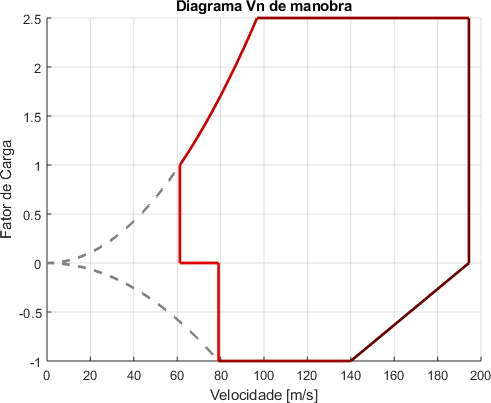
\includegraphics[width=0.75\textwidth]{images/parte3/diagramavn_asalimpa.png}
\caption[Diagrama Vn]{Diagrama Vn}
\label{fig:diagramavn}
\end{figure}

\begin{table}[H]
\centering
\begin{tabular}{cccc}
\toprule
Velocidade & Descrição & Definição & Valor \\ \midrule
$V_{S_{+}}$ & Velocidade de estol & $ \sqrt{\frac{2 W}{\rho S C_{L_{max}}}} $ & 61.33 m/s \\ [0.3cm]
 & positivo (asa limpa) & &  \\ [0.3cm]
$V_A$ & Velocidade de Manobra & $ V_{S_{+}} \sqrt{n_{max}} $ & 96.97 m/s \\ [0.3cm]
$V_C$ & Velocidade de Cruzeiro & Requisito & 140 m/s \\  [0.3cm]
$V_H$ & Velocidade Horizontal & $V_C/0.9$ & 155.56 m/s \\  [0.3cm]
 & Máxima & &  \\ [0.3cm]
$V_D$ & Velocidade de Mergulho & $1.25 V_C$ & 194.44 m/s \\ [0.3cm]
$V_{S_{-}}$ & Velocidade de estol & $ \sqrt{\frac{2 W}{\rho S C_{L_{min}}}} $ & 79.17 m/s \\ [0.3cm]
 & negativo (asa limpa) & &  \\ [0.3cm]
\bottomrule
\end{tabular}
\caption[Velocidades de Projeto - Asa Limpa]{Velocidades de Projeto - Asa Limpa}
\label{tbl:velocidadesprojeto}
\end{table}

\subsection{Principais Derivadas Longitudinais}
\label{derivadas}

As derivadas aerodinâmicas foram estimadas a partir de ábacos disponíveis em ETKIN e pela modelagem aerodinâmica discutida na \autoref{superf_sustentadoras}. Os valores apresentados na \autoref{tbl:derivadas} são os valores finais dado a atualização da geometria da empenagem horizontal e são os valores usados nas análises seguintes.

\begin{table}[H]
\centering
\begin{tabular}{cccc}
\toprule
$ \frac{\partial C_{L_{asa}}}{\partial \alpha} $ & 4.586 & $ \frac{\partial C_{L_{eh}}}{\partial \alpha} $ & 3.566 \\ [0.3cm]
$ \frac{\partial C_{L_{eh}}}{\partial \eta} $ & 1.837 & $ \frac{\partial C_{L_{eh}}}{\partial \delta_{tab}} $ & 1.097 \\ [0.3cm]
$ \frac{\partial C_{H_{eh}}}{\partial \alpha} $ & -0.0967  & $ \frac{\partial C_{H_{eh}}}{\partial \eta} $ & -0.4246 \\ [0.3cm]
$ \frac{\partial C_{H_{eh}}}{\partial \delta_{tab}} $ & -0.2015 & $ \frac{\partial \epsilon}{\partial \alpha} $ & 0.1352 \\ [0.3cm]
\bottomrule
\end{tabular}
\caption[Principais Derivadas Longitudinais]{Principais Derivadas Longitudinais}
\label{tbl:derivadas}
\end{table}

\section{Margem Estática Longitudinal}
\label{margem}

O cálculo da margem estática longitudinal é função do ponto neutro como descrito pela \autoref{eqmargemestatica}.

\begin{equation}
\label{eqmargemestatica}
K_n = - \frac{\partial C_m}{\partial \widetilde{C_L}} = h_n - h
\end{equation}

\begin{description}
\item[$K_n$  -] Margem estática longitudinal
\item[$h_n$ -] Posição do ponto neutro em relação a CMA
\item[$h$ -] Posição do CG em relação a CMA
\item[$\frac{\partial C_m}{\partial \widetilde{C_L}}$ -] Derivada do momento de arfagem no CG pelo coeficiente de sustentação devido a pertubação
\end{description}

Já o ponto neutro é cálculo a partir de duas hipóteses:


\textbf{Manche Fixo}: não há deflexão de profundor com uma pertubação qualquer.

\begin{equation}
h_n = h_0 + \frac{\overline{V} a_1 \epsilon_{\alpha}}{a}
\end{equation}

\begin{description}
\item[$h_0$  -] Posição do CA em relação a CMA
\item[$\overline{V}$ -] Volume de cauda horizontal
\item[$\epsilon_{\alpha}$ -] Downwash
\item[$a_1$ -] Variação do coeficiente de sustentação da empenagem horizontal com ângulo de ataque
\item[$a$ -] Variação do coeficiente de sustentação da aeronave com ângulo de ataque
\end{description}

\textbf{Manche Livre}: a força que o piloto faz no manche é constante com as pertubações, ou seja, não há variação no momento de articulação do profundor

\begin{equation}
h_n = h_0 + \frac{ \overline{V} \overline{a_1} \epsilon_{\alpha} }{a}
\end{equation}

\begin{equation}
\overline{a_1} =  a_1 - \frac{a_2}{b_2} b_1
\end{equation}

\begin{description}
\item[$a_2$ -] Variação do coeficiente de sustentação da empenagem horizontal com deflexão do profundor
\item[$b_1$ -] Variação do coeficiente de momento na articulação do profundor com ângulo de ataque
\item[$b_2$ -] Variação do coeficiente de momento na articulação do profundor com deflexão do profundor
\end{description}

No caso, a aeronave é considerada de médio porte sendo desejável a atuação das superfícies de controle através de um sistema hidráulico. Dessa forma, a hipotése de manche livre é extremamente improvável, logo considera-se como limitante a condição de manche fixo apesar de ser calculado a condição de manche livre para fins de comparação.

O passeio de CG necessário definido na análise de passeio de CG realizada anteriormente fornecem os limites do CG utilizados na analise de estabilidade. O valor da distância entre o centro aerodinâmico da asa e da empenagem horizontal foi atualizado sendo seu valor final menor que o previamente utilizado. Portanto, para atender ao requisito de passeio de CG, houve um aumento de área de empenagem horizontal para compensar a diminuição de $l_t$ além de um aumento visando aumentar a margem estática longitudinal para CG traseiro.

A \autoref{tbl:comparacao_empenagens} apresenta uma comparação entre a geometria da empenagem estimada inicialmente e a geometria refinada da empenagem juntamente com o ponto neutro manche fixo estimado para cada configuração.

\begin{table}[H]
\centering
\begin{tabular}{ccc}
\toprule
$ Empenagem $ & Geometria Inicial & Geometria Refinada \\
$ l_t $ & 13.5m & 12.255m \\
$ S $ & 7.1 $m^2$ & 8.9 $m^2$ \\
$ \overline{V} $ & 0.9 & 1.2 \\
$ h_n $ & 0.2800 & 0.3056 \\
$ K_n $ & 3.0\% & 5.6\% \\
\bottomrule
\end{tabular}
\caption[Comparação entre geometria inicial e geometria refinada da empenagem horizontal]{Comparação entre geometria inicial e geometria refinada da empenagem horizontal}
\label{tbl:comparacao_empenagens}
\end{table}

Por fim, a \autoref{tbl:ponto_neutro} resume os valores de ponto neutro mache fixo e manche livre para a geometria refinada da empenagem horizontal. Já a \autoref{tbl:margem_estatica} apresenta os valores finais para a margem estática considerando os limites de CG. O critério inicialmente adotado para a margem estática mínima foi de 5\% considerando que um sistema \textit{fly-by-wire} de aumento de estabilidade pode ser implementado na aeronave nos trabalhos futuros caso necessário.

\begin{table}[H]
\centering
\begin{tabular}{cc}
\toprule
$ h_n $ & 0.3056 \\
$ h_n' $ & 0.2933 \\
\bottomrule
\end{tabular}
\caption[Ponto Neutro]{Ponto Neutro}
\label{tbl:ponto_neutro}
\end{table}

\begin{table}[H]
\centering
\begin{tabular}{ccc}
\toprule
CG & Traseiro & Dianteiro \\ \midrule
$ K_n $ & 5.56\% & 30.56\% \\
$ K_n' $ & 4.33\% & 29.33\% \\
\bottomrule
\end{tabular}
\caption[Margem Estática Longitudinal]{Margem Estática Longitudinal}
\label{tbl:margem_estatica}
\end{table}

A margem estática manche fixo é positiva e maior que o critério de 5\% o que constata que a aeronave em projeto é estaticamente estável no passeio de CG definido para operação.

\section{Controle Longitudinal - Profundor}
\label{controlelongitudinal}

A análise de controle longitudinal é pautada na carga no atuador representado pelo \textit{hinge moment} da superfície e pelos batentes de deflexão devido a atuação das superfícies de controle por um sistema hidráulico. Definido o escopo, avaliou-se duas opções de profundor considerando formato elíptico do bordo de ataque:

\begin{enumerate}
\item Profundor correspondente a 20\% da corda da empenagem horizontal

\item Profundor correspondente a 30\% da corda da empenagem horizontal
\end{enumerate}

A comparação entre ambas foi realizada considerando critérios como proximidade com os batentes de deflexão da superfície de controle e magnitude do \textit{hinge moment} (momento de articulação) visando reduzir carga no atuador. Os batentes de deflexão foram definidos a partir de valores típicos encontrados e estão apresentados na \autoref{tbl:batentes}.

\begin{table}[H]
\centering
\begin{tabular}{cc}
\toprule
Batente positivo & 17\textdegree\ \\
Batente negativo & -23\textdegree\ \\
\bottomrule
\end{tabular}
\caption[Batentes de deflexão do profundor]{Batentes de deflexão do profundor}
\label{tbl:batentes}
\end{table}

Do ponto de vista de carga no atuador, o \textit{hinge moment} foi calculado para manter voo reto e nivelado de acordo com o envelope de velocidades apresentado pela aeronave no CG dianteiro no MTOW. O equacionamento desta condição de voo é dado pelas equações \ref{voo1g_1} a \ref{voo1g_7} e a \autoref{fig:comp_hingemoment} mostra o resultado obtido para o \textit{hinge moment}.

% EQUAÇÕES - VOO TRIMADO 1G
\begin{equation}
\label{voo1g_1}
\overline{\eta} =  A_1 \overline{C_L} + A_2
\end{equation}

\begin{equation}
\label{voo1g_2}
A_1 = \frac{(h - h_0) - \overline{V} a_1 frac{\epsilon_{\alpha}}{a} }{ \overline{V} a_2}
\end{equation}

\begin{equation}
\label{voo1g_3}
A_2 = \frac{C_{m_0} - \overline{V} a_1 i_t - \overline{V} a_3 \delta}{\overline{V} a_2}
\end{equation}

\begin{equation}
\label{voo1g_4}
\overline{M_H} =  B_1 + B_2 V^2
\end{equation}

\begin{equation}
\label{voo1g_5}
B_1 = \frac{(h - h_0) - \overline{V} \overline{a_1} frac{\epsilon_{\alpha}}{a} }{ \overline{V} a_2} b_2 \frac{W}{S} S_{\eta} \overline{c_{\eta}}
\end{equation}

\begin{equation}
\label{voo1g_7}
B_2 = 0.5 \rho S_{\eta} \overline{c_{\eta}} (b_0 + b_2 (\frac{C_{m_0} - \overline{V} a_1 i_t - \overline{V} \overline{a_3} \delta}{\overline{V} a_2}))
\end{equation}

\begin{equation}
\overline{a_3} = a_3 + \frac{a_1}{b_1} b_3
\end{equation}


\begin{description}
\item[$\overline{\eta}$ -] Deflexão de profundor para manter voo reto e nivelado
\item[$\overline{M_H}$ -] hinge moment para voo reto e nivelado
\item[$a_3$ -] Variação do coeficiente de sustentação da empenagem horizontal com deflexão do compensador (tab)
\item[$b_0$ -] É nulo no caso de perfis assimétricos (NACA0012)
\item[$b_3$ -] Variação do coeficiente de momento na articulação do profundor com deflexão do compensador (tab)
\end{description}

\begin{figure}[H]
\centering
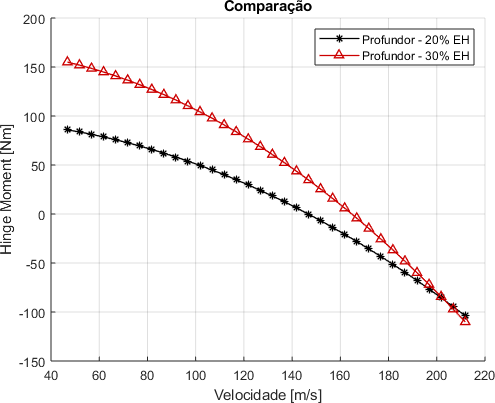
\includegraphics[width=0.75\textwidth]{images/parte3/comparacao_hingemoment.png}
\caption[Comparação de \textit{Hinge Moment} entre diferentes profundores em tamanho]{Comparação de \textit{Hinge Moment} entre diferentes profundores em tamanho para voo reto e nivelado e CG dianteiro}
\label{fig:comp_hingemoment}
\end{figure}

Como pode ser observado, o profundor menor apresenta um \textit{hinge moment} menor ao longo do envelope de velocidade evidenciando um benefício em sua escolha.

A \autoref{fig:comp_def} apresenta o resultado obtido a partir das derivadas aerodinâmicas para a deflexão de profundor necessária para realização de uma manobra longitudinal equilibrada no fator de carga máximo, CG dianteiro e MTOW. O equacionamento desta condição de voo é dado pelas equações \ref{margemmanobra1} a \ref{vooNz_4}.

% EQUAÇÕES MARGEM DE MANOBRA
\begin{equation}
\label{margemmanobra1}
H_m = h_0 + \overline{V} a_1 (\epsilon_{\alpha}/a + 1/2 \mu) - h
\end{equation}

\begin{equation}
\label{margemmanobra2}
H_m' = h_0 + \overline{V} \overline{a_1} (\epsilon_{\alpha}/a + 1/2 \mu) - h
\end{equation}

\begin{equation}
\label{margemmanobra3}
\mu = \frac{W}{g \rho l_t' S}
\end{equation}

\begin{description}
\item[$H_m$ -] Margem de Manobra considernado hipótese de manche fixo
\item[$H_m'$ -] Margem de Manobra considernado hipótese de manche livre
\item[$l_t'$ -] Distância do CG da aeronave até o centro aerodinâmico da empenagem
\end{description}

% EQUAÇÕES MANOBRA EQUILIBRADA
\begin{equation}
\label{vooNz_1}
\eta' = \overline{\eta} + \Delta\overline{\eta}
\end{equation}

\begin{equation}
\label{vooNz_2}
\Delta\overline{\eta} = - \frac{H_m}{\overline{V} a_2} (n - 1) \overline{C_L}
\end{equation}

\begin{equation}
\label{vooNz_3}
M_H' = \overline{M_H} + \Delta\overline{M_H}
\end{equation}

\begin{equation}
\label{vooNz_4}
\Delta\overline{M_H} = - \frac{W}{S} S_{\eta} \overline{c_{\eta}} \frac{b_2}{\overline{V} a_2} H_m' (n-1)
\end{equation}

\begin{description}
\item[$M_H'$ -] Hinge moment necessário para executar manobra
\item[$\eta'$ -] Deflexão de profundor necessára para executar manobra
\end{description}

\begin{figure}[H]
\centering
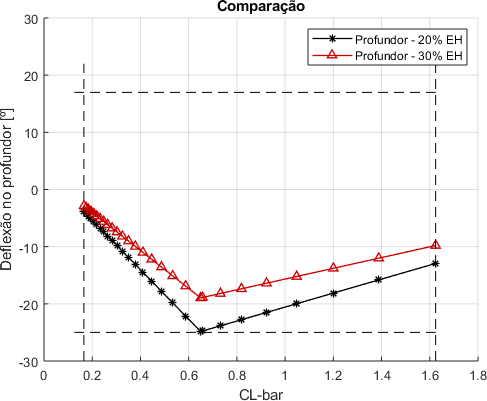
\includegraphics[width=0.75\textwidth]{images/parte3/comparacao_deflexao.png}
\caption[Comparação de Deflexão entre diferentes profundores em tamanho para manobra equilibrada]{Comparação de Deflexão entre diferentes profundores em tamanho para manobra equilibrada no fator de carga máximo e CG dianteiro}
\label{fig:comp_def}
\end{figure}

Como pode ser observado, o profundor corresponde a 20\% da corda da empenagem horizontal atinge o batente de deflexão negativa enquanto que a outra opção apresenta uma deflexão maxima de 78\% o valor do batente. Nessa primeira comparação, um profundor menor se mostra mais adequado. As análises seguintes consideram apenas o profundor final - 20\% da corda da empenagem horizontal.

As margens de manobra para as posições de CG definidas em \autoref{margem} são calculadas a partir das equações \ref{margemmanobra1} a \ref{margemmanobra3} e os resultados são apresentados na tabela \autoref{tbl:margem_manobra}.

\begin{table}[H]
\centering
\begin{tabular}{ccc}
\toprule
CG & Traseiro & Dianteiro \\ \midrule
$ H_m $ & 12.58\% & 37.72\% \\
$ H_m' $ & 10.52\% & 35.65\% \\
\bottomrule
\end{tabular}
\caption[Margem de Manobra Longitudinal]{Margem de Manobra Longitudinal}
\label{tbl:margem_manobra}
\end{table}

As margens de manobra são positivas o que indica a capacidade da aeronave de realizar manobras equilibradas longitudinais.

A partir das equações \ref{voo1g_1} a \ref{voo1g_7}, é possível determinar as deflexões de profundor para voo de cruzeiro considerando os limites de CG definidos em \autoref{margem} e MTOW. A \autoref{fig:def_voo1g} apresenta o resultado obtido.

\begin{figure}[H]
\centering
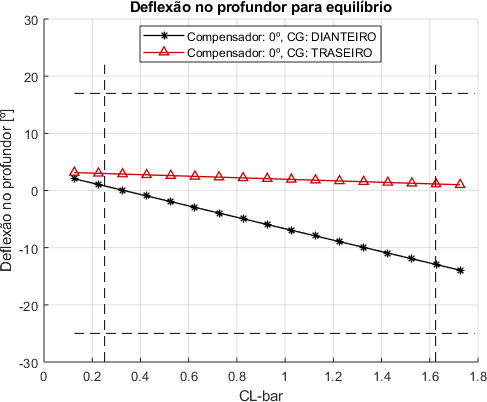
\includegraphics[width=0.75\textwidth]{images/parte3/De_equi_c20.png}
\caption[Deflexão de profundor para voo reto e nivelado]{Deflexão de profundor para voo reto e nivelado}
\label{fig:def_voo1g}
\end{figure}

A inclinação negativa das curvas é característica de uma aeronave estaticamente estável.

As equações equações \ref{vooNz_1} a \ref{vooNz_4} permitem a determinção das deflexões de profundor para manobra equilibrada considerando os limites de CG definidos em \autoref{margem}, o diagrama vn definido em \label{diagramavn} e MTOW. A \autoref{fig:def_vooNz} apresenta o resultado obtido.

\begin{figure}[H]
\centering
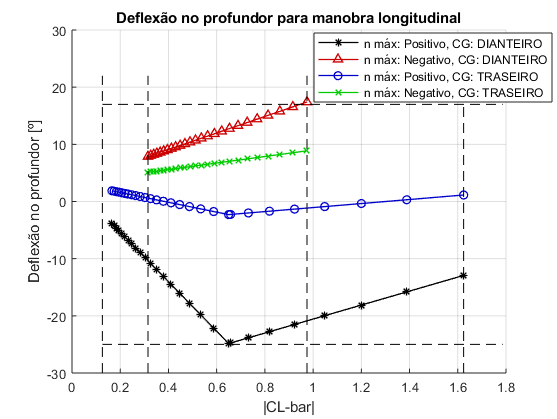
\includegraphics[width=0.75\textwidth]{images/parte3/De_man_c20.png}
\caption[Deflexão de profundor para manobra equilibrada]{Deflexão de profundor para manobra equilibrada}
\label{fig:def_vooNz}
\end{figure}

Como pode ser observado na monobra equilibrada longitudinal considerando os extremos de fator de carga e limites de CG, o profundor atinge ambos os batentes positivo e negativo o que comprova a escolha adequada da superfície de controle. Esse resultado foi possível ao se ajustar a incidência da empenagem horizontal para -3\textdegree\ .
